% !TeX spellcheck = en_US
\documentclass{beamer}

\mode<presentation> {
	\usetheme{Berkeley}
}

\usepackage[english]{babel}
\usepackage{lipsum}
\usepackage{natbib}
\usepackage{url}
\usepackage[utf8x]{inputenc}
\usepackage{amsmath}
\usepackage{graphicx}
\usepackage{parskip}
\usepackage{fancyhdr}
\usepackage{vmargin}
\usepackage{listings}
\usepackage{hyperref}

\graphicspath{{images/}}


\title[Sprint Review]{ROW5 Sprint 4 Review}

\author{ROW Team 5}
\institute[HvA]
{
	Amsterdam University of Applied Sciences \\
	\textit{https://rescueonwheels.github.io/}
}
\date{Januari 14, 2019}

\begin{document}
	\begin{frame}
		\titlepage
	\end{frame}

	\section{Introduction}
In the (near) future robots will be more and more part of our daily life. Even more than they are already part of society today. Industrial robots are nowadays very common, the use of drones by military and civilians triggers discussion and science is creating robots to take care of people who need help. Functioning more or less autonomous requires that such machines have to be robust, take their own decisions and operate in a safe way. 

Thus we created a robot that helps to rescue people trapped in a collapsed building.

The user is able to control the robot using the combination of a controller, specifically a Steam Controller, and a moblie phone as display used by the Google Cardboard. Of course, being a robot, the robot itself wants to do as much as possible. The degree of autonomy of the robot has been focused on assisting the user as much as possible.

	\begin{frame}{Overview}
	\tableofcontents
\end{frame}

	\section{Sensors and actuators}

\begin{frame}{\secname}
	Sensor(s):
	\begin{itemize}
		\item Distance sensor (ultrasonic sensor HC-SR04).
	\end{itemize}

	Actuator(s):
	\begin{itemize}
		\item Custom double axis servo platform.
	\end{itemize}

	Other:
	\begin{itemize}
		\item Fisheye lens.
	\end{itemize}
\end{frame}

	\section{Communication}

\begin{frame}{\secname}
	Rover $\leftrightarrow$ Cockpit:
	\begin{itemize}
		\item Socket.IO.
	\end{itemize}

	Rover $\rightarrow$ Tincidunt:
	\begin{itemize}
		\item H.264 over HTTP.
	\end{itemize}

	Cockpit $\leftarrow$ Controller:
	\begin{itemize}
		\item Bluetooth;
		\item USB.
	\end{itemize}
\end{frame}

	\section{User Interface}

\begin{frame}{\secname: Epicenter}
	\begin{center}
		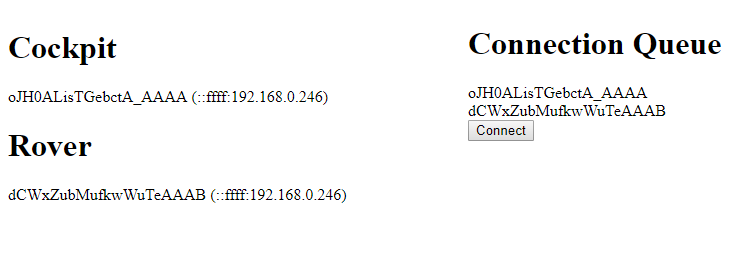
\includegraphics[width=\linewidth]{images/epicenter.png}
	\end{center}
\end{frame}

\begin{frame}{\secname: Chrome}
	\begin{center}
		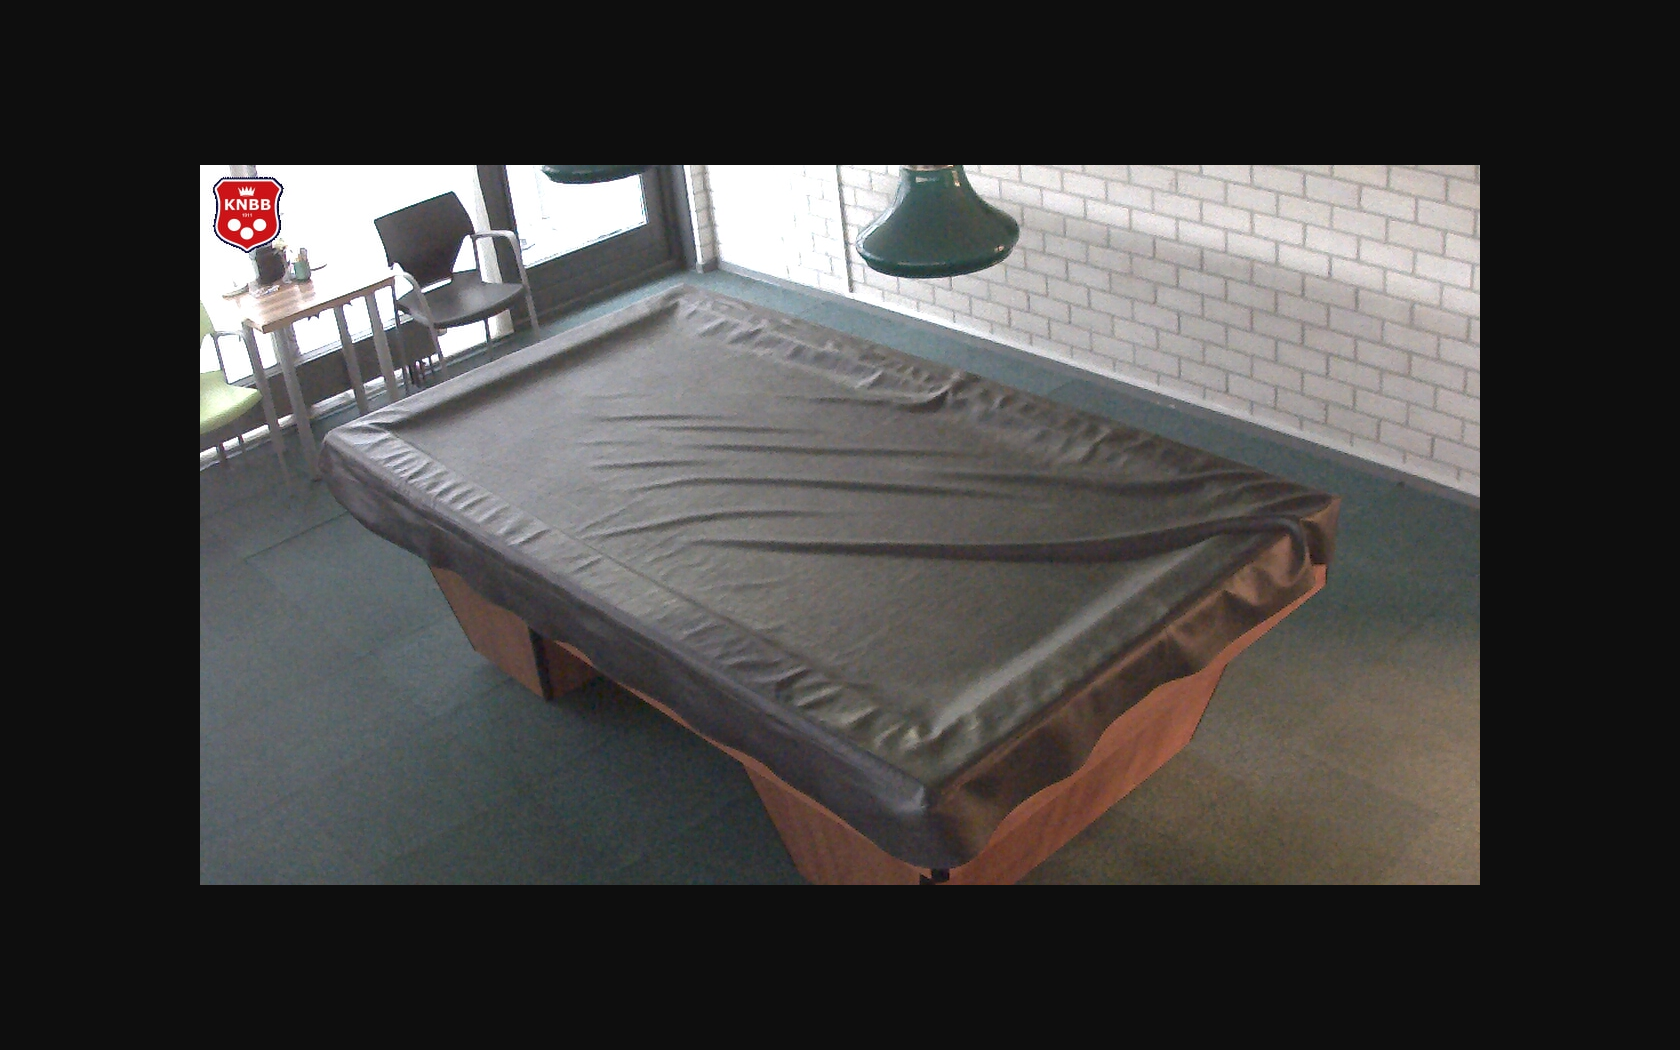
\includegraphics[width=\linewidth]{images/chrome.png}
	\end{center}
\end{frame}

\begin{frame}{\secname: Tincidunt}
	\begin{center}
		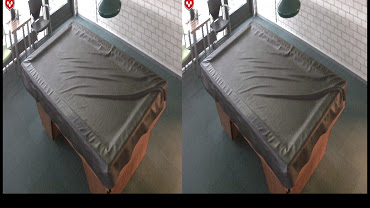
\includegraphics[width=\linewidth]{images/tincidunt.png}
	\end{center}
\end{frame}

	\section{Operational scenario}

\begin{frame}{\secname}
	TODO
\end{frame}

	\section{Documentation}

\begin{frame}{\secname}
	\begin{itemize}
		\item Rover Rescue System - Business Case
		\item Rover Rescue System - (Technical) Documentation
		\item Rover Rescue System - Manual - Application
		\item Rover Rescue System - Manual - Epicenter
		\item Rover Rescue System - Manual - Rover
		\item Rover Rescue System - Project File
	 	\item Rover Rescue System - Sprint Review 1
	 	\item Rover Rescue System - Sprint Review 2
	 	\item Rover Rescue System - Sprint Review 3
	 	\item Rover Rescue System - Sprint Review 4
 	\end{itemize}
\end{frame}

	\section{Innovatation}

\begin{frame}{\secname}
	\begin{itemize}
		\item Virtual Reality as video output;
		\item Virtual Reality connected to the camera;
		\item Automated prevention systems:
		\begin{itemize}
			\item Auto-stop to prevent crashes;
			\item Auto-stop based on communication events;
			\item Auto-reset of camera view based on communication events;
			\item Scalable for large scale operations.
		\end{itemize}
	\end{itemize}
\end{frame}

	\section{Scrum}

\begin{frame}{\secname}
	\begin{itemize}
		\item Use of GitHub projects;
		\item Use of GitHub because of third-party integrations;		
		\item Use of ZenHub for automated issue tracking;
		\begin{itemize}
			\item Isssues
			\item Epics
			\item Pull Requests
		\end{itemize}
		\item Use of ZenHub for Burndown and Velocity tracking;
	\end{itemize}
\end{frame}

\begin{frame}{\secname: Cumulative Flow}
	\begin{center}
		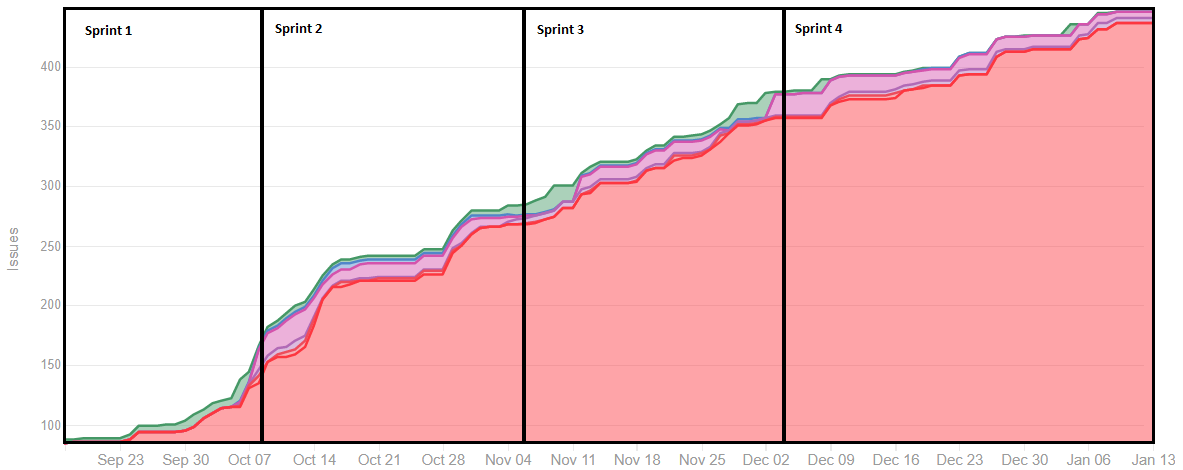
\includegraphics[width=\linewidth]{images/flow.png}
	\end{center}
\end{frame}

\begin{frame}{\secname: Burndown sprint 1}
	\begin{center}
		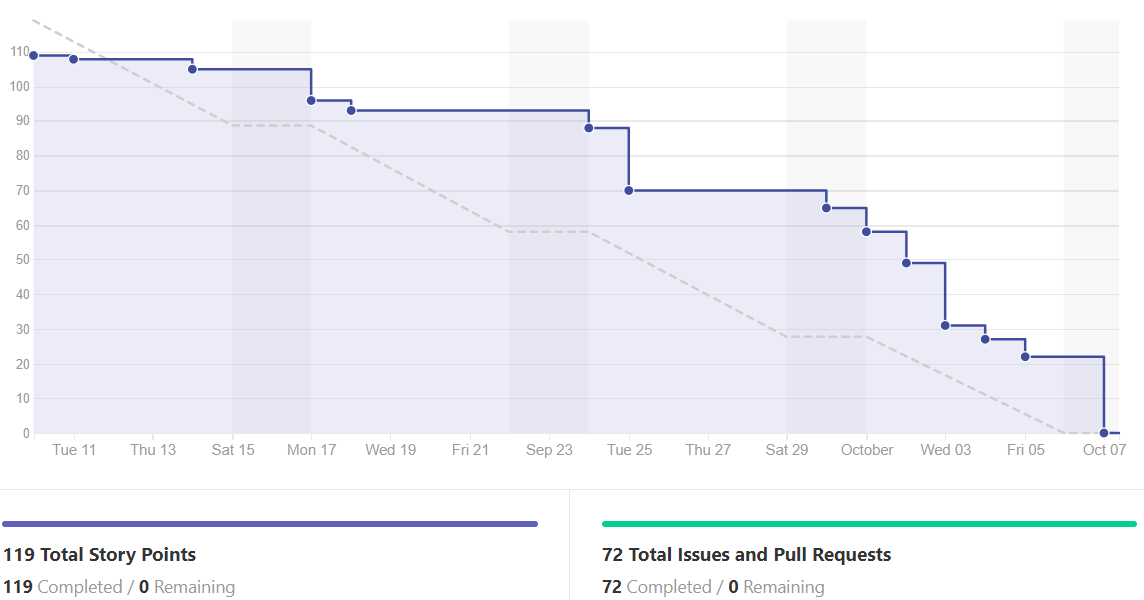
\includegraphics[width=\linewidth]{images/burn1.png}
	\end{center}
\end{frame}

\begin{frame}{\secname: Burndown sprint 2}
	\begin{center}
		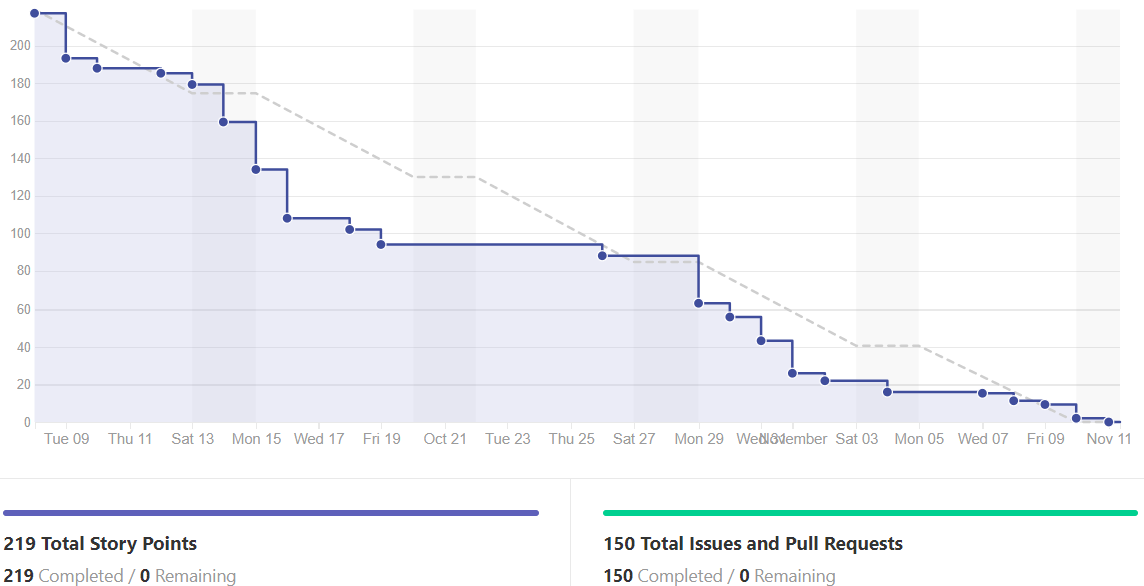
\includegraphics[width=\linewidth]{images/burn2.png}
	\end{center}
\end{frame}

\begin{frame}{\secname: Burndown sprint 3}
	\begin{center}
		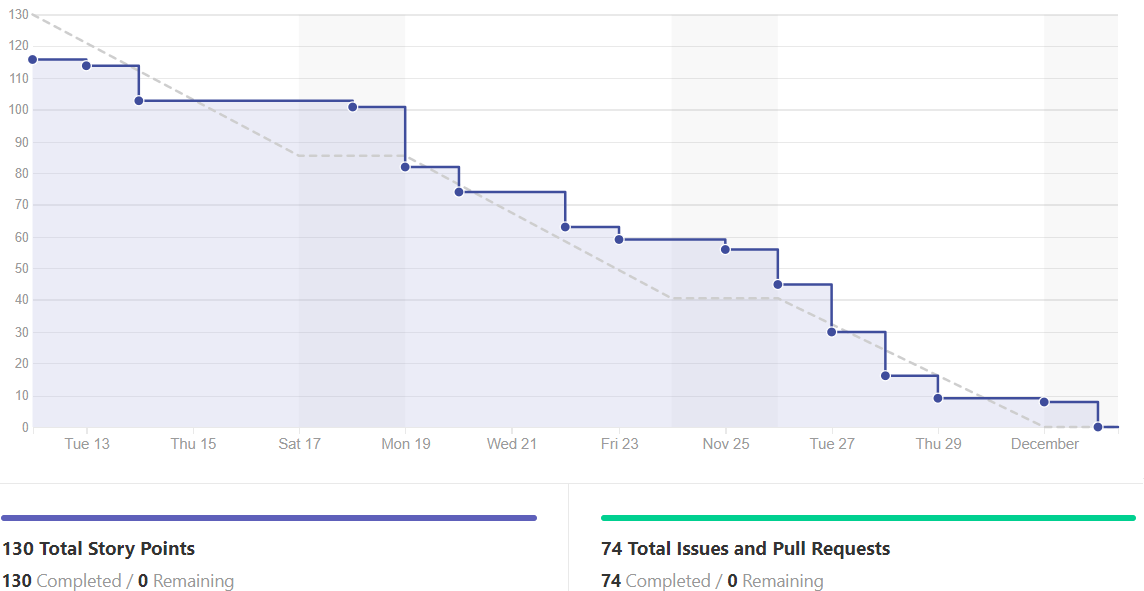
\includegraphics[width=\linewidth]{images/burn3.png}
	\end{center}
\end{frame}

\begin{frame}{\secname: Burndown sprint 4}
	\begin{center}
		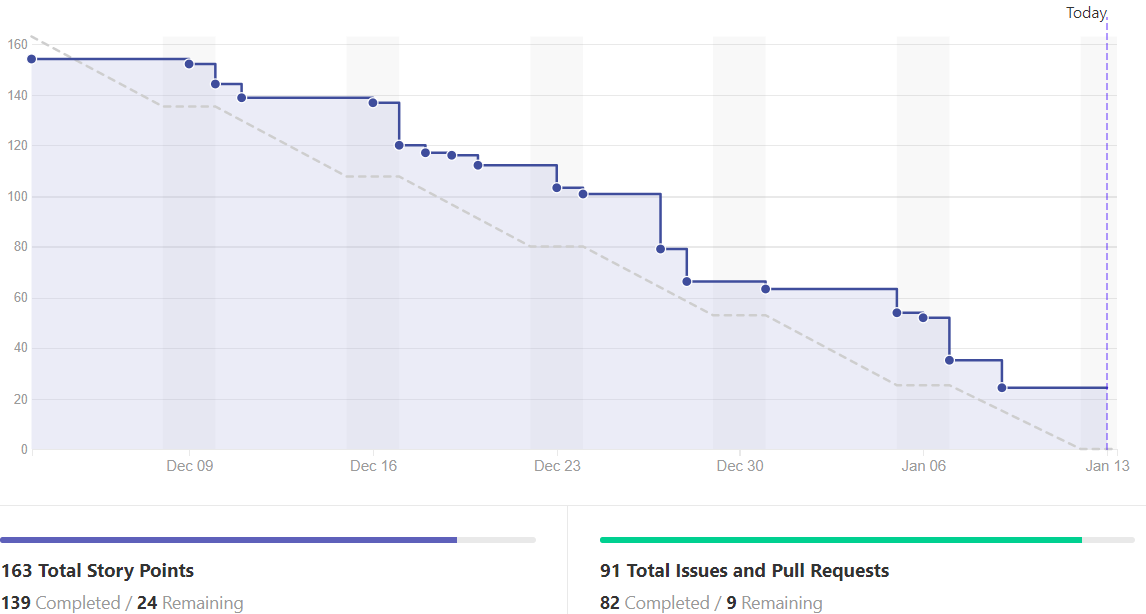
\includegraphics[width=\linewidth]{images/burn4.png}
	\end{center}
\end{frame}

	\section{Quality assurance}

\begin{frame}{\secname}
	\begin{itemize}
		\item Use of GIT submodules;
		\item Custom mocks for simulation usage;
		\item Protected branches with following rules:
			\begin{itemize}
				\item Require pull request reviews before merging;
				\item Require status checks to pass before merging
				\begin{itemize}
					\item Travis-CI used for tests and code style;
					\item CodeClimate used for unbiased code quality;
					\item Coveralls is used for code coverage.
				\end{itemize}
			\end{itemize}
		\item Definition of Done;
		\item Definition of Ready.
	\end{itemize}
\end{frame}

	\section{End}

\begin{frame}
	\Huge{\centerline{Any Questions?}}
\end{frame}

\begin{frame}
	\Huge{\centerline{The End}}
\end{frame}

\end{document}